\section{Задание движения твёрдого тела через углы Эйлера}

\begin{figure}[H]
  \centering
  \resizebox{\linewidth}{!}{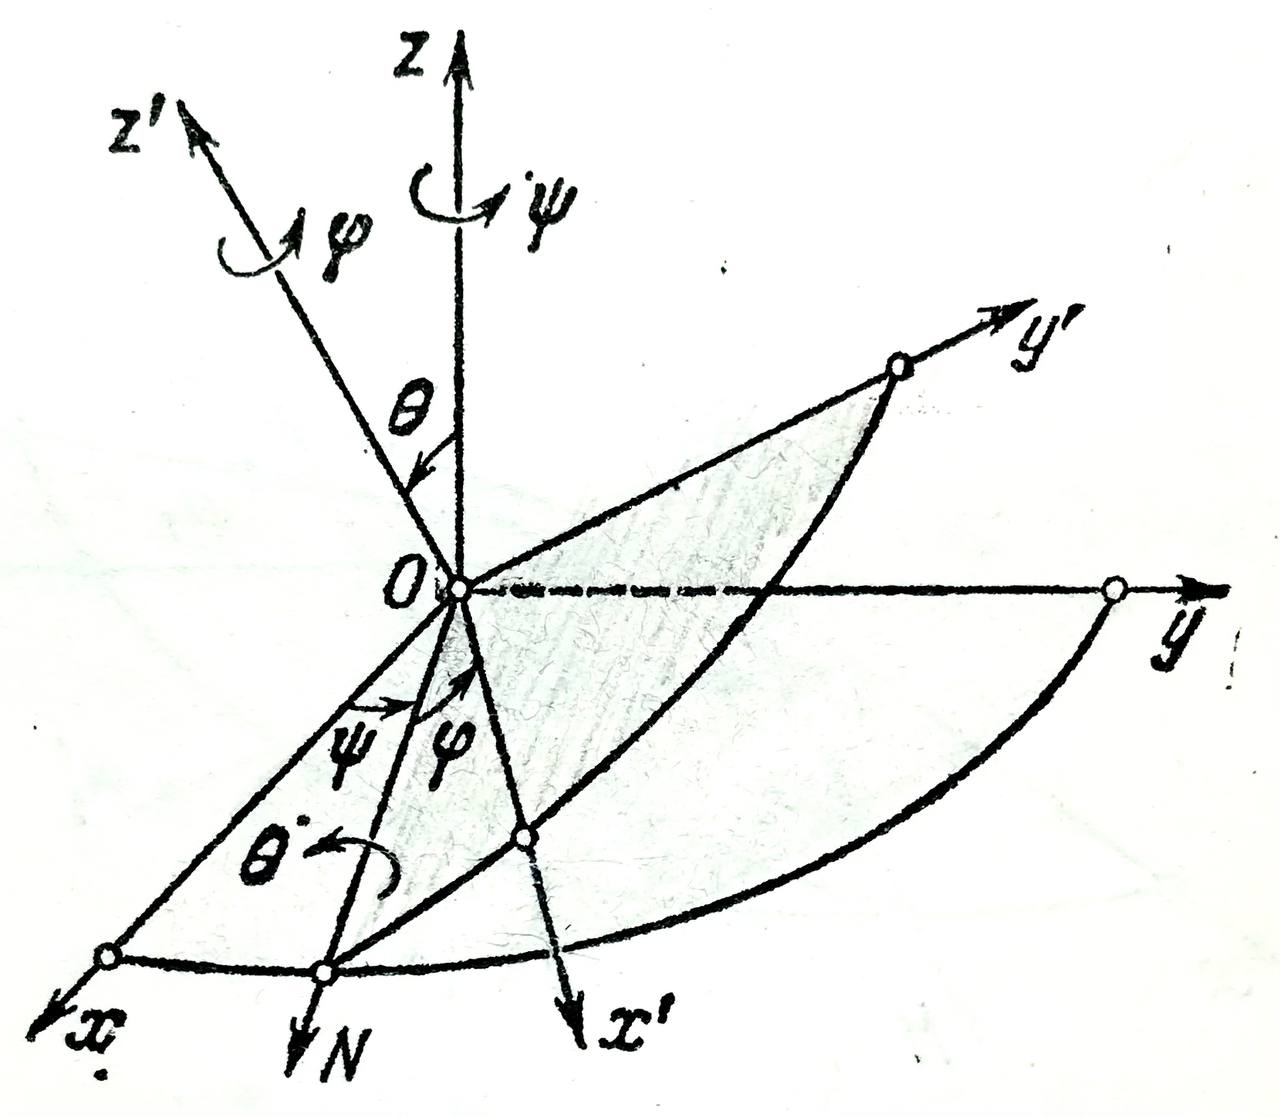
\includegraphics{src/mechanics/pictures/19_1.jpg}}

  \caption{}
  \label{fig:19_1}
\end{figure}

Соединим жёстко с вращающимся телом подвижную систему координат $Ox'y'z'$ и
будем рассматривать вращение этой системы по отношению к неподвижной системе
$Oxyz$. Введём таблицу косинусов углов между осями координат:
\begin{equation*}
  \begin{array}{|c|c|c|c|}
    \hline
    & x & y & z \\
    \hline
    x' & p_{11} & p_{12} & p_{13} \\
    \hline
    y' & p_{21} & p_{22} & p_{23} \\
    \hline
    z' & p_{31} & p_{32} & p_{33} \\
    \hline
  \end{array}
\end{equation*}

Связь между координатами точки $M$ в подвижной и неподвижной системах:
\begin{equation}
  \label{eq:coords_transform}
  \begin{aligned}
    \left(
    \begin{array}{c}
      x \\
      y \\
      z \\
    \end{array}
    \right)
    &=
    \left(
    \begin{array}{c c c}
      p_{11} & p_{12} & p_{13} \\
      p_{21} & p_{22} & p_{23} \\
      p_{31} & p_{32} & p_{33}
    \end{array}
    \right)
    \left(
    \begin{array}{c}
      x' \\
      y' \\
      z' \\
    \end{array}
    \right), \\
    \left(
    \begin{array}{c}
      x' \\
      y' \\
      z' \\
    \end{array}
    \right)
    &=
    \left(
    \begin{array}{c c c}
      p_{11} & p_{21} & p_{31} \\
      p_{12} & p_{22} & p_{32} \\
      p_{13} & p_{23} & p_{33}
    \end{array}
    \right)
    \left(
    \begin{array}{c}
      x \\
      y \\
      z \\
    \end{array}
    \right).
  \end{aligned}
\end{equation}

Отметим линию $ON$ пересечения плоскостей $xOy$ и $x'Oy'$ и назовём её
\textit{линией узлов}. Выберём на этой линии положительное направление $ON$ так,
чтобы, смотря с него, видеть вращение оси $Oz$ к оси $Oz'$ на наименьший угол в
положительном направлении (то есть в правой системе осей --- против часовой
стрелки); легко видеть, плоскость $zOz'$ перпендикулярна к оси $ON$.

Первый эйлеров угол --- угол \textit{прецессии} $\psi$ --- образован в плоскости
$xOy$ линией узлов с неподвижной осью $Ox$; отсчитывается угол $\psi$ в
положительном направлении (по часовой стрелке) от оси $Ox$ к оси $ON$, если
смотреть с оси $Oz$.

Второй угол --- угол \textit{нутации} $\theta$ --- расположен в плоскости $zOz'$
и отсчитывается от оси $Oz$ к оси $Oz'$ в положительном направлении (против
часовой стрелки), если смотреть с положительного направления оси $ON$.

Третий угол --- угол \textit{ротации}, или угол \textit{чистого вращения}
$\varphi$ --- расположен в плоскости $x'Oy'$, причём отсчитывается от линии
узлов $ON$ до оси $Ox'$ в положительном направлении.

\begin{figure}[H]
  \centering
  \resizebox{\linewidth}{!}{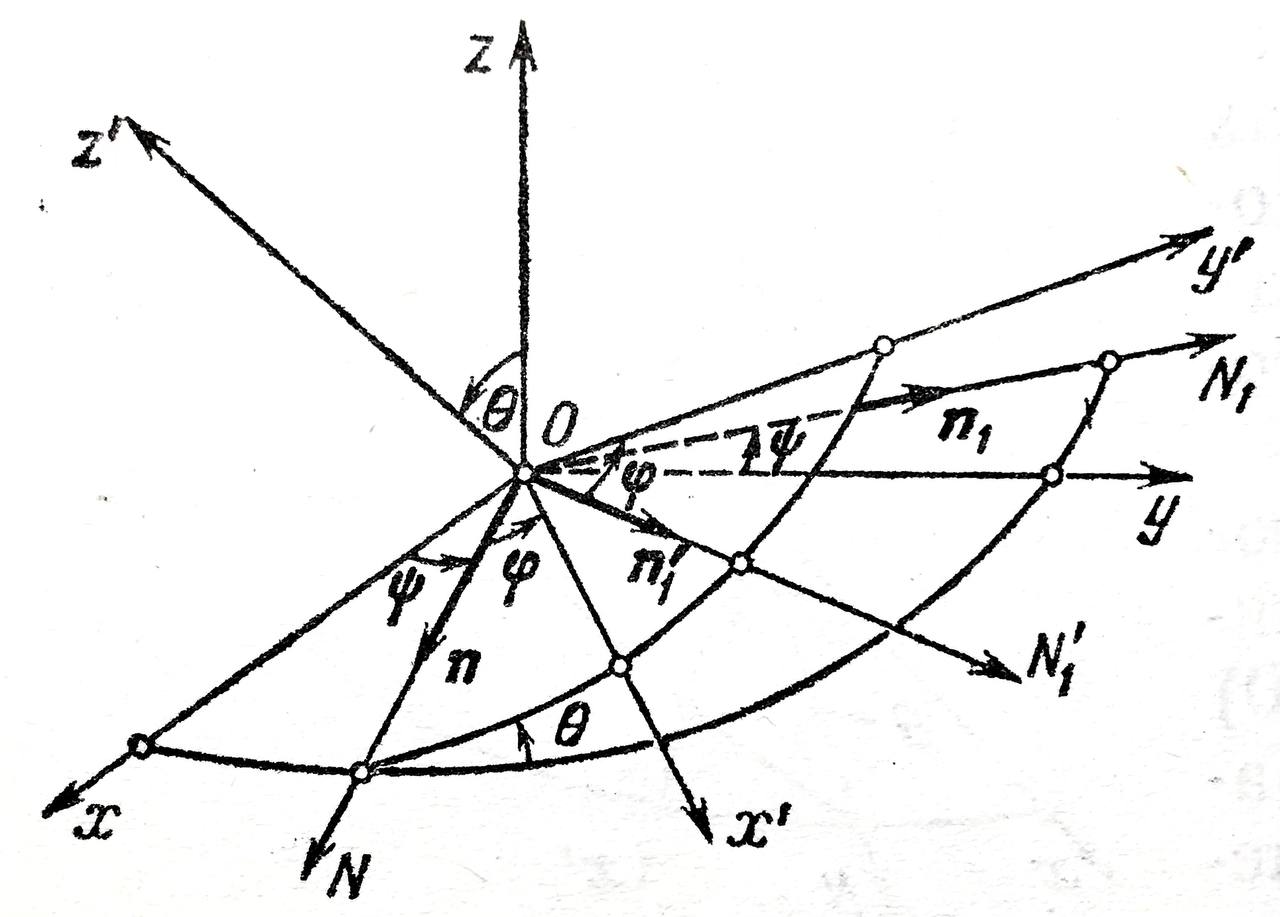
\includegraphics{src/mechanics/pictures/19_2.jpg}}

  \caption{}
  \label{fig:19_2}
\end{figure}

Для установления зависимостей между косинусами углов осей координат и эйлеровыми
углами применим следующий приём. Введём, кроме единичных векторов осей координат
$\vec{i}, \vec{j}, \vec{k}, \pvec{i}, \pvec{j}, \pvec{k}$, ещё единичные векторы
следующих осей:
\begin{itemize}
  \item $\vec{n}$ --- линии узлов $ON$;
  \item $\vec{n}_1$ --- оси $ON_1$, перпендикулярной к оси $ON$ и лежащей в
    плоскости $xOy$;
  \item $\pvec{n}_1$ --- оси $ON_1'$, перпендикулярной к оси $ON$ и лежащей в
    плоскости $x'Oy'$.
\end{itemize}

Направление оси $ON_1$ выберем так, чтобы оси $ONN_1 z$ образовали триэдр,
сонаправленный (то есть правый) с системой осей $Oxyz$; направление оси $ON_1'$
выберем так, чтобы оси $ONN_1' z'$ образовали сонаправленный триэдр с системой
$Ox'y'z'$, а следовательно, и с системой $Oxyz$. Легко видеть, что угол между
осями $ON_1'$ и $ON_1$ представляет собой линейный угол двугранного угла между
плоскостями $x'Oy'$ и $xOy$, то есть угол $\theta$ (\textcolor{red}{TODO:} не
помню, есть ли в билетах определение линейного угла двугранного угла...).
Тогда, замечая ещё, что единичные векторы $\vec{i},~\vec{j}$ и $\pvec{i},~
\pvec{j}$ легко могут быть выражены через единичные векторы $\vec{n},~\vec{n}_1$
и $\pvec{n}_1$ в форме зависимостей, получаемых из разложения одних единичных
векторов по другим:
\begin{equation}
  \begin{aligned}
    \vec{i} &= \phantom{-} \vec{n} \cos\psi - \vec{n}_1 \sin\psi, \\
    \vec{j} &= \phantom{-} \vec{n} \cos\varphi + \pvec{n}_1 \sin\varphi, \\
    \vec{i} &= \phantom{-} \vec{n} \sin\psi + \vec{n}_1 \cos\psi, \\
    \vec{i} &= -\vec{n} \sin\varphi + \pvec{n}_1 \cos\varphi, \\
  \end{aligned}
\end{equation}
найдём
\begin{equation*}
  \begin{aligned}
    p_{11} &= \dotprod{\vec{i}}{\pvec{i}} \\
      &= \dotprod{
        \paren{\vec{n} \cos\psi - \vec{n}_1 \sin\psi}
      }{
        \paren{\vec{n} \cos\varphi + \pvec{n}_1 \sin\varphi}
      } \\
      &= \phantom{-}
        (\dotprod{\vec{n}}{\vec{n}}) \cos\psi \cos\varphi +
        (\dotprod{\vec{n}}{\pvec{n}_1}) \cos\psi \sin\varphi - \\
      &\phantom{=} -
        (\dotprod{\vec{n}_1}{\vec{n}}) \sin\psi \cos\varphi -
        (\dotprod{\vec{n}_1}{\pvec{n}_1}) \sin\psi \sin\varphi.
  \end{aligned}
\end{equation*}
Имеем
\begin{equation*}
  \dotprod{\vec{n}}{\vec{n}} = 1, \quad
  \dotprod{\vec{n}}{\pvec{n}_1} = 0, \quad
  \dotprod{\vec{n}_1}{\vec{n}} = 0, \quad
  \dotprod{\vec{n}_1}{\pvec{n}_1} = \cos\theta,
\end{equation*}
откуда
\begin{equation*}
  p_{11} = \cos\psi \cos\varphi - \sin\psi \sin\varphi \cos\theta.
\end{equation*}
Аналогично получим остальные косинусы.

Выделим полученную группу формул:
\begin{equation}
  \label{eq:euler_cos}
  \begin{aligned}
    p_{11} &= \cos(\widehat{x, x'})
      = \phantom{-} \cos\psi \cos\varphi - \sin\psi \sin\varphi \cos\theta, \\
    p_{21} &= \cos(\widehat{x, y'})
      = -\cos\psi \sin\varphi - \sin\psi \cos\varphi \cos\theta, \\
    p_{31} &= \cos(\widehat{x, z'})
      = \phantom{-} \sin\psi \sin\theta, \\
    p_{12} &= \cos(\widehat{y, x'})
      = \phantom{-} \sin\psi \cos\varphi + \cos\psi \sin\varphi \cos\theta, \\
    p_{22} &= \cos(\widehat{y, y'})
      = -\sin\psi \sin\varphi + \cos\psi \cos\varphi \cos\theta, \\
    p_{32} &= \cos(\widehat{y, z'})
      = -\cos\psi \sin\theta, \\
    p_{13} &= \cos(\widehat{z, x'})
      = \phantom{-} \sin\varphi \sin\theta, \\
    p_{23} &= \cos(\widehat{z, y'})
      = \phantom{-} \cos\varphi \sin\theta, \\
    p_{33} &= \cos(\widehat{z, z'})
      = \phantom{-} \cos\theta.
  \end{aligned}
\end{equation}

\begin{theorem}
  Пусть
  \begin{equation*}
    \begin{aligned}
      P &= \left(
        \begin{array}{c c c}
          p_{11} & p_{21} & p_{31} \\
          p_{12} & p_{22} & p_{32} \\
          p_{13} & p_{23} & p_{33}
        \end{array}
        \right), \\
      P_1(t) &= \left(
      \begin{array}{c c c}
        1 & 0 & 0 \\
        0 & \cos t & -\sin t \\
        0 & \sin t & \phantom{-} \cos t
      \end{array}
      \right), \\
      P_2(t) &= \left(
      \begin{array}{c c c}
        \cos t & -\sin t & 0 \\
        \sin t & \phantom{-} \cos t & 0 \\
        0 & 0 & 1
      \end{array}
      \right).
    \end{aligned}
  \end{equation*}
  Тогда
  \begin{equation}
    P = P_2(\psi) P_1(\theta) P_2(\varphi).
  \end{equation}
\end{theorem}

\begin{proof}
  Равенство проверяется перемножением матриц.

  Можно также доказать, используя геометрический смысл преобразований (поворот).

  % TODO
  (\textcolor{red}{TODO:} доказать поворотами?)
\end{proof}

\subsection{Список литературы}
\begin{enumerate}
  \item \cite{lourie}
\end{enumerate}

